\documentclass[pdftex]{article}
\usepackage[T1]{fontenc}
\usepackage[utf8]{inputenc}
\usepackage{graphicx}
\usepackage[font=scriptsize,labelfont=bf]{caption}
\usepackage{titling}

\setlength{\droptitle}{-15em}
\title{PHYS 723 Homework 7}
\author{Nick Tyler}
\date{}


\begin{document}
\captionsetup[figure]{aboveskip=-15pt}
\captionsetup[figure]{belowskip=15pt}
\maketitle
\begin{enumerate}
	\item  Here is a histogram showing the number of particles by events.\\
	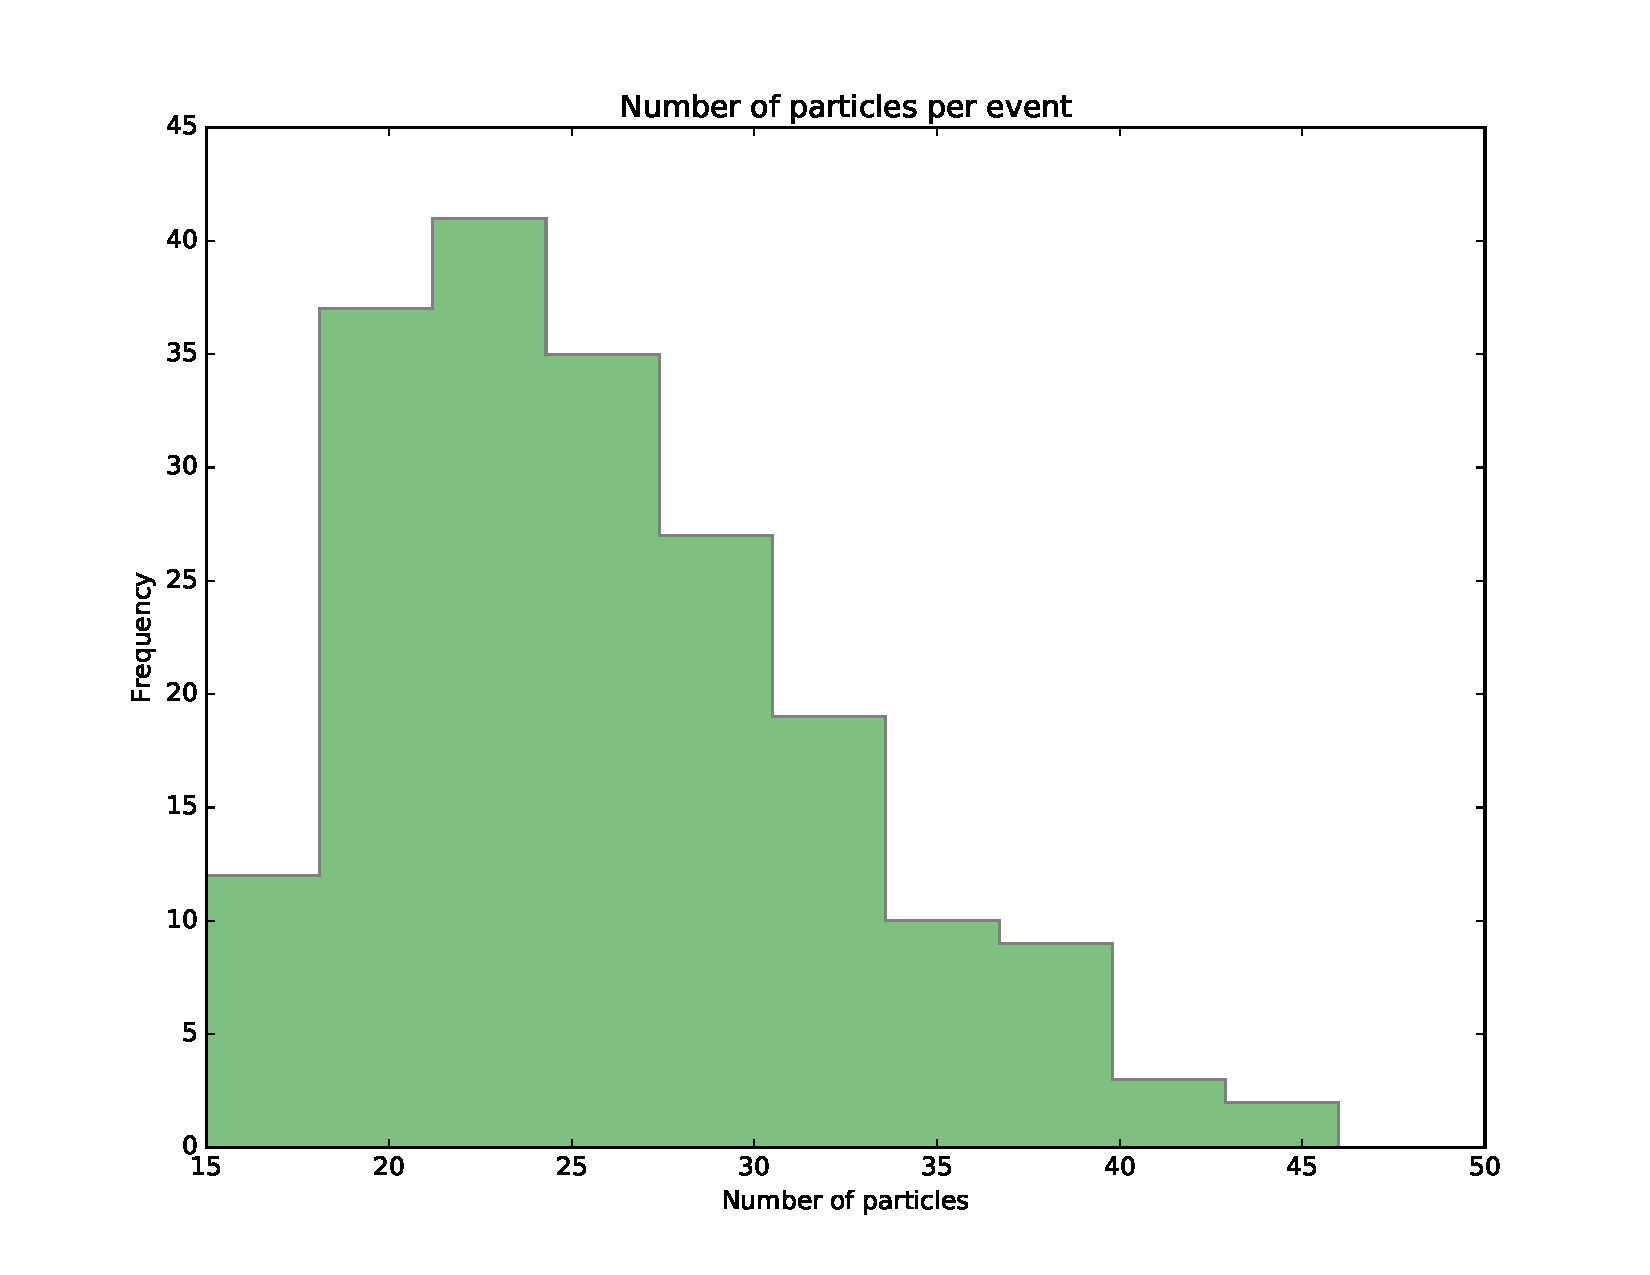
\includegraphics[scale=0.4]{Number_of_particles.pdf}\\
	\captionof{figure}{Here is a histogram showing the number of particles by events.}


	\item Here is a histogram of the momentum in the X direction of all $\pi^+$ and $\pi^-$. \\ 
	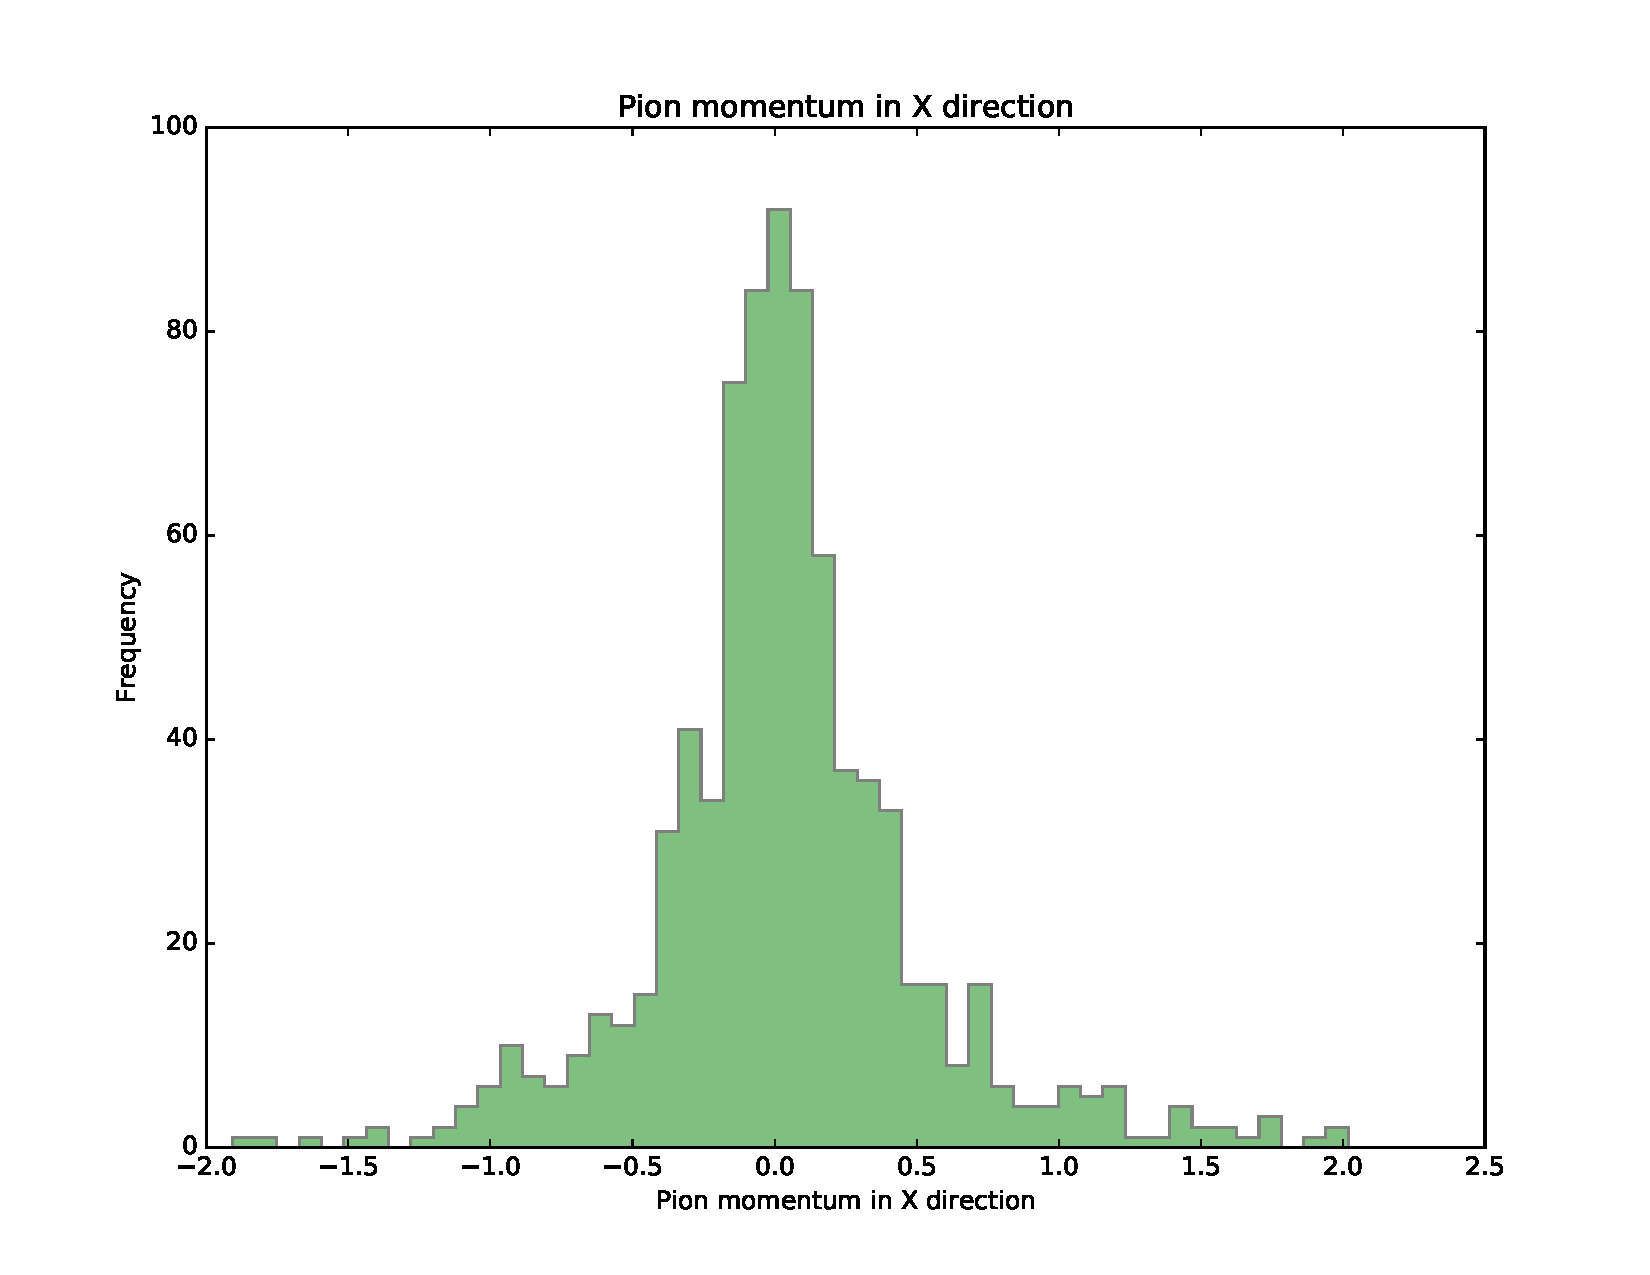
\includegraphics[scale=0.4]{Pion_px.pdf}\\
	\captionof{figure}{$P_x$ for $\pi^+$ and $\pi^-$}




\end{enumerate}

\end{document}
